

%\documentclass[aip,reprint]{revtex4-1}
%\documentclass[aip,jap,preprint]{revtex4-1}
\documentclass[a4paper,fleqn]{cas-sc}

%\usepackage{mdframed}
%\usepackage{color}
%\usepackage{enumitem}

\usepackage[numbers]{natbib}
\usepackage{mdframed}
\usepackage{color}
\usepackage{enumitem}
\usepackage[most]{tcolorbox}
\usepackage{soul}

\begin{document}
\shorttitle{}

\tcbset{highlight style/.style={
  colback=yellow, colframe=yellow, boxrule=0pt, sharp corners, enhanced,
  left=0mm, right=0mm, top=0mm, bottom=0mm
}}

\sethlcolor{yellow}

Dear Editor and Reviewers,

We sincerely thank you for taking the time to review our manuscript
``Extracting the iron concentration in silicon solar cells using photovoltaic parameters and machine learning''
(Ms. Ref. No.: SEJ-D-25-01089).
Your insightful comments and constructive suggestions have greatly helped us improve
the quality of our work.
We particularly appreciate your careful reading and thoughtful feedback,
which have led to significant improvements in both the technical content and presentation clarity of our manuscript.
We have carefully addressed all the comments and made corresponding revisions to the manuscript.
The location of revisions is pointed by red color and highlighted in yellow in ``MarkedManuscript.pdf''.
Below we provide our detailed point-by-point responses to each comment.
We hope the revised manuscript better meets your expectations and standards for publication in Solar Energy.
%The location of revisions is pointed by blue color in ``MarkedManuscript.pdf''.

\subsection*{Response to Reviewer \#1 }

\noindent
\textcolor[rgb]{0.00,0.50,1.00}{\textbf{Comment~1.}}
\emph{The introduction lacks the role of iron valency (ferrous or ferric) in silicon solar cells.}

\noindent
\textcolor[rgb]{0.51,0.00,0.00}{\textbf{Reply:}}

Reviewer is correct that ferrous (Fe$^{2+}$) and ferric (Fe$^{3+}$) states deserve consideration,
as they are the most common and stable charge states of iron.
These ionic forms typically occur in compounds where iron forms chemical bonds (either ionic or covalent) with other elements,
as well as in cases where iron is present as an impurity in solid materials.
In silicon, iron can also exist in a trivalent (ferric) state when it substitutes for a silicon atom at a lattice site.
However, under normal conditions, the concentration of substitutional iron is extremely low, less than 1\% of the total iron impurity atoms \cite{Wright2016}.
Increasing the concentration of substitutional iron requires special sample processing, such as high-temperature annealing or irradiation.
Moreover, substitutional iron acts as a weak recombination center,
so its influence on the properties of silicon solar cells can be neglected.
The ferrous form is virtually absent in silicon.
The majority of iron impurity atoms in silicon occupy positions,
where they can exist in either a neutral (Fe$_i^0$) or positively charged (Fe$_i^+$) state,
depending on the position of the Fermi level \cite{Istratov1999}.
In $n$-type silicon,Fe$_i$ is more likely to exist in a neutral state,
whereas in $p$-type silicon, it is more likely to be positively charged.
Even when interstitial iron forms complex point defects, such as iron–boron pairs (Fe$_i$B$_s$), no valence bonds are formed.
In interstitial configuration, iron acts as an active recombination center.

Consequently, in silicon solar cells, the role of iron valence is negligible,
in contrast to other types of solar cells, such as perovskite solar cells \cite{Poindexter2017}.
Specifically, in MAPbI$_3$-based devices, both Fe$^{3+}$ and Fe$^{2+}$  point defects are observed,
with Fe$^{3+}$ being electronically inactive in terms of recombination.

We have added the relevant information to the Introduction (page 2, third paragraph from the top).


%\begin{mdframed}
%(ii)~iron is one of the most prevalent, ubiquitous, and efficiency-limiting metallic impurities \cite{Buonassisi2006, IronSC}.
%
%%\colorbox{yellow}{
%\begin{tcolorbox}[highlight style]
%\textcolor[rgb]{1.00,0.07,0.00}{
%It is well known that ferrous (Fe$^{2+}$) and ferric (Fe$^{3+}$) are the most common and stable charge states of iron in most materials.
%But the majority of iron impurity atoms in silicon occupy interstitial positions,
%where they can exist in either a neutral (Fe$_i^0$) or positively charged (Fe$_i^+$) state,
%depending on the position of the Fermi level \cite{Macdonald2004,Istratov1999}.
%In $n$-type silicon,Fe$_i$ is more likely to exist in a neutral state,
%whereas in $p$-type silicon, it is more likely to be positively charged.
%Even when interstitial iron forms complex point defects no valence bonds are formed.
%In silicon, iron can also exist in a trivalent (ferric) state when it substitutes for a silicon atom at a lattice site.
%However, under normal conditions, the concentration of substitutional iron is extremely low, less than 1\% of the total iron impurity atoms \cite{Wright2016}.
%The ferrous form is virtually absent in silicon.
%Consequently, in silicon solar cells, the role of iron valence is negligible,
%in contrast to other photovoltaic technologies, such as perovskite-based devices \cite{Poindexter2017}.}%}
%\end{tcolorbox}
%
%It is well established that in $p$-type material,
%iron tends to bind with dopant atoms such as boron,
%\end{mdframed}

\vspace{1cm}
\noindent
\textcolor[rgb]{0.00,0.50,1.00}{\textbf{Comment~2.}}
\emph{The work didn't deal with the redox reaction of iron in silicon solar cells.}

\noindent
\textcolor[rgb]{0.51,0.00,0.00}{\textbf{Reply:}}

Initially, it is important to note that
redox reactions do not play a central role in silicon solar cells,
unlike dye-sensitized solar cells or photoelectrochemical cells.
However, changes in the charge states of individual atoms --- whether intrinsic or impurity-related ---
occur during the photoelectric conversion process.
For example, during the recombination of charge carriers at iron-related defects
(such as interstitial iron atoms or iron-boron pairs),
electron capture occurs in the initial stage:
\begin{eqnarray*}
  \mathrm{Fe}_i^++e^-&\rightarrow& \mathrm{Fe}_i^0\,, \\
  (\mathrm{Fe_iB_s})^0+e^-&\rightarrow& (\mathrm{Fe_iB_s})^-\,,
\end{eqnarray*}
which typically corresponds to a reduction reaction.
In the subsequent stage, hole capture alters the defect's charge state again
\begin{eqnarray*}
  \mathrm{Fe}_i^0+h^+&\rightarrow& \mathrm{Fe}_i^+\,, \\
  (\mathrm{Fe_iB_s})^-+h^+&\rightarrow& (\mathrm{Fe_iB_s})^0\,,
\end{eqnarray*}
formally representing an oxidation reaction.
When FeB pairs dissociate due to intense illumination, electron injection, or heating up to 200~$^\circ$C,
the iron atom becomes neutral by capturing an electron (reduction) during the first step of this two-stage process.
After dissociation and the cessation of the external stimulus,
the interstitial iron atom loses an electron (oxidation),
becoming singly positively charged, which allows it to re-form a pair with a negatively charged dopant (boron).
However, transitions between different charge states of iron-related defects in silicon
are governed by electron and hole capture and emission processes,
involving the exchange of carriers between the defect levels and the conduction or valence band.
These processes are described within Shockley–Read–Hall theory
and do not constitute redox reactions in the classical chemical sense.

Consequently, the original manuscript did not emphasize redox reactions of iron in silicon solar cells,
and the Reviewer’s observation is valid.
In the revised manuscript, we have included a note on the distinct nature of charge-state transitions in iron-related defects,
highlighting how they differ from classical redox reactions (page 2, fourth paragraph from the top).

%\begin{mdframed}
%It is well established that in $p$-type material,
%iron tends to bind with dopant atoms such as boron, forming iron–boron pairs under equilibrium conditions
%or existing as interstitial species only in the presence of sufficiently high free electron densities \cite{Kimerling1983, FeBAssJAP2014}.
%The deliberate transition between these states can be readily induced
%through intense illumination, electron injection, or heating up to 200~$^\circ$C and
%is commonly employed in various methods for assessing iron concentration
%\cite{Zoth1990, Rein2, Schmidt2005, Goodarzi2017, Olikh2021JAP, FeMethod2012, Herguth2022, Macdonald2004}.
%\textcolor[rgb]{1.00,0.07,0.00}{
%\hl{
%It is worth noting that the charge-state transitions of iron-related defects ---
%whether during recombination activity or FeB pair dissociation --- formally resemble redox reactions.
%However, these processes involve the exchange of charge carriers between defect levels and the conduction or valence band,
%are governed by Shockley–Read–Hall theory, and are not described by classical redox chemistry.
%}}
%\end{mdframed}

\vspace{1cm}
\noindent
\textcolor[rgb]{0.00,0.50,1.00}{\textbf{Comment~3.}}
\emph{In the title, "Extracting the iron concentration" should be changed to "Determination of iron concentration.}

\noindent
\textcolor[rgb]{0.51,0.00,0.00}{\textbf{Reply:}}

We concur that the phrase ``Determination of iron concentration'' better emphasizes the quantitative aspect
of the work and aligns well with the standard terminology used in similar studies.
Accordingly, we have revised the manuscript title to:
``Determination of iron concentration in silicon solar cells using photovoltaic parameters and machine learning.''


\vspace{1cm}
\subsection*{Response to Reviewer \#2 }

\noindent
\textcolor[rgb]{0.00,0.50,1.00}{\textbf{Comment~1.}}
\emph{Why temperature range (290-340)~K?
what was the dissociation efficiency of FeB pairs at this temperature?
How much is translated to cell degradation?
Since at this temperature range, other factors also go side on that impact device characteristic.}


\noindent
\textcolor[rgb]{0.51,0.00,0.00}{\textbf{Reply:}}

We hope that the proposed approach will be applied to evaluate the concentration of iron in already installed solar modules
and during the certification of photovoltaic converters.
On the one hand, the selected temperature range of 290–340~K reflects the typical operating conditions of most silicon solar cells.
On the other hand, the IEC 61215-2:2021 \cite{IEC61215} standard requires that temperature coefficients of
short-circuit current, open-circuit voltage, and maximum power be determined based on current–voltage measurements conducted
within a temperature range of approximately +15~$^\circ$C to +75~$^\circ$C (288–348~K).
In other words, the standard solar cell testing results can serve as input data for machine learning models trained within selected temperature range.

Additional information justifying the choice of temperature range has been added in the revised manuscript (page 4, first paragraph).


Complete dissociation of the FeB pairs was achieved during experiments conducted within the specified temperature range
(further clarified below in response to the following Reviewer's comment).


The changes in photovoltaic parameter values resulting from FeB pair dissociation depend on
both the concentration of iron impurities and the solar cell parameters
(such as base thickness and dopant concentration),
as well as the measurement conditions (illumination intensity and spectral composition, temperature).
This issue is discussed in more detail in \cite{Olikh2025MSEB},
which presents the results of silicon solar cell modeling used to create the training dataset.
For instance, under AM1.5 illumination, the relative changes in short-circuit current range
from $-40.88$\%
(for $N_\mathrm{B}=10^{17}$~cm$^{-3}$, $T=290$~K, $d_p=380$~$\mu$m)
to 6.11\%
(for $N_\mathrm{B}=10^{15}$~cm$^{-3}$, $T=315$~K, $d_p=380$~$\mu$m).
Similarly, the relative changes in open-circuit voltage vary from
$-12.95$\%
(for $N_\mathrm{B}=10^{15}$~cm$^{-3}$, $T=340$~K, $d_p=180$~$\mu$m)
to 1.92\%
(for $N_\mathrm{B}=1.778\times10^{15}$~cm$^{-3}$, $T=340$~K, $d_p=230$~$\mu$m).
Notably, the most pronounced changes in solar cell characteristics do not necessarily occur at the highest iron concentrations.
For example, the maximum negative change in open-circuit voltage ($-12.95$\%)
is observed at an iron concentration of $3.162\times10^{12}$~cm$^{-3}$,
rather than at the highest tested level.

This suggests that FeB pair dissociation, depending on the specific parameters,
can not only degrade solar cell performance but also improve certain characteristics \cite{Olikh2025MSEB,FeB:Schmidt}.
However, it is important to emphasize that light-induced dissociation of FeB pairs does not lead to irreversible changes in photovoltaic parameters.
Once the illumination ceases, the FeB pairs re-form, and the solar cell characteristics return to their original values \cite{FeBLight2,FeBAssJAP2014,FeBKin2019,FeMethod2012,FeBLight2,FeBAssJAP2014}.


Information regarding the ranges of changes in photovoltaic parameters and their reversibility has been added to the revised manuscript
(page 4, third paragraph from the top; page 3, first paragraph in Section~2.1).

We fully agree with the Reviewer that, within the chosen temperature range,
factors beyond iron concentration and the selected descriptors may also influence solar cell characteristics.
This is especially relevant for real solar cells, which, in addition to iron,
may contain other recombination-active impurities.
To better isolate iron-related effects from the influence of other factors,
we used relative changes in PV parameters as model inputs.
Since models trained in this way provided sufficiently accurate predictions of iron concentration from
both simulated and experimentally measured current–voltage characteristics, we consider this approach well justified.


\vspace{1cm}
\noindent
\textcolor[rgb]{0.00,0.50,1.00}{\textbf{Comment~2.}}
\emph{Complete details about the dissociation of FeB pairs using halogen lamp illumination? What was the time duration? How much was the decay efficiency.}

\noindent
\textcolor[rgb]{0.51,0.00,0.00}{\textbf{Reply:}}

It is known \cite{Macdonald2004} that strong optical illumination ($>$100~W/m$^{2}$)
results in almost complete (>99\%) dissociation of the FeB pairs.
The dissociation rate $R_d$ is influenced by the pair concentration $N_\mathrm{FeB}$ and overall carrier generation rate $G$, which is proportional to the illumination intensity
\cite{FeBLight2,FeBAssJAP2014,FeBKin2019,FeMethod2012}:
\begin{equation}
\label{eqRd}
R_d=K\left(\frac{G}{N_\mathrm{FeB}}\right)^2\,,
\end{equation}
where
$K$ is the constant of the material.
Additionally, it is well established that $R_d$ depends on temperature \cite{Lagowskii1993,lauer2016},
the spectral composition of illumination \cite{OlikhPSSA},
and the presence of recombination channels other than those associated with iron-related defects \cite{FeBLight2,FeBAssJAP2014}.

For experimental validation of the proposed models, samples with an iron concentration of $2\times10^{11}$ to $4\times10^{13}$~cm$^{-3}$ were used.
Dissociation of FeB pairs was induced by intense illumination from a halogen lamp (7000~W/m$^{2}$).
The illumination duration required to achieve near-complete dissociation depended on the iron concentration
and reached up to 400~s for the solar cell with the highest $N_\mathrm{FeB}$ values.
When selecting the illumination intervals, we considered the results of a previous study \cite{OlikhPSSA},
which showed that in samples with a similar defect composition and exposed to a comparable light source,
complete dissociation at $N_\mathrm{Fe}=9\times10^{12}$~cm$^{-3}$ occurred within 20~s.

Details regarding the selection of the illumination duration can be found on page 3 (last paragraph).




\vspace{1cm}
\noindent
\textcolor[rgb]{0.00,0.50,1.00}{\textbf{Comment~3.}}
\emph{Most of the models significantly fail for the AM1.5 illumination? What could be the reason for that?}

\noindent
\textcolor[rgb]{0.51,0.00,0.00}{\textbf{Reply:}}

Indeed, models trained on data obtained under AM1.5 illumination perform worse in almost all cases.
We believe this can be attributed to the following reasons.
It is well known that a regression model may  achieve high accuracy
by having the target variable be an unambiguous function of the descriptor.
Moreover, the absolute value of the function’s derivative should be as significant as possible.
As shown earlier  \cite{Olikh2025MSEB}, the condition of uniqueness in the relationship between $N_\mathrm{Fe}$ and
the changes in photovoltaic parameters under AM1.5 illumination is often not fulfilled in contrast to the case of monochromatic illumination.
In addition, the ranges of changes in $\varepsilon I_\mathrm{SC}$, $\varepsilon V_\mathrm{OC}$, and $\varepsilon \eta$
under monochromatic illumination exceed those observed under AM1.5 illumination.
For illustration, Fig.~\ref{fig1} shows some examples from  \cite{Olikh2025MSEB}.
The physical origin of the differences in the relationship between iron concentration and
parameter changes under AM1.5 and monochromatic illumination lies in the fact that,
in the former case, the generation of non-equilibrium charge carriers occurs throughout the
entire volume of the solar cell, rather than being limited to the base region.
As a result, the processes involved in photovoltaic conversion are more complex.
In our view, these differences explain why the performance of ML models trained on AM1.5 illumination data is generally poorer.
One way to address the ambiguity in the relationship between features and the target variable
is to incorporate additional features into the model.
As shown in the study (e.g., see Fig.~7 in manuscript),
for AM1.5 illumination, increasing the number of descriptors often improves prediction accuracy, supporting our hypothesis.



\begin{figure}
	\centering
     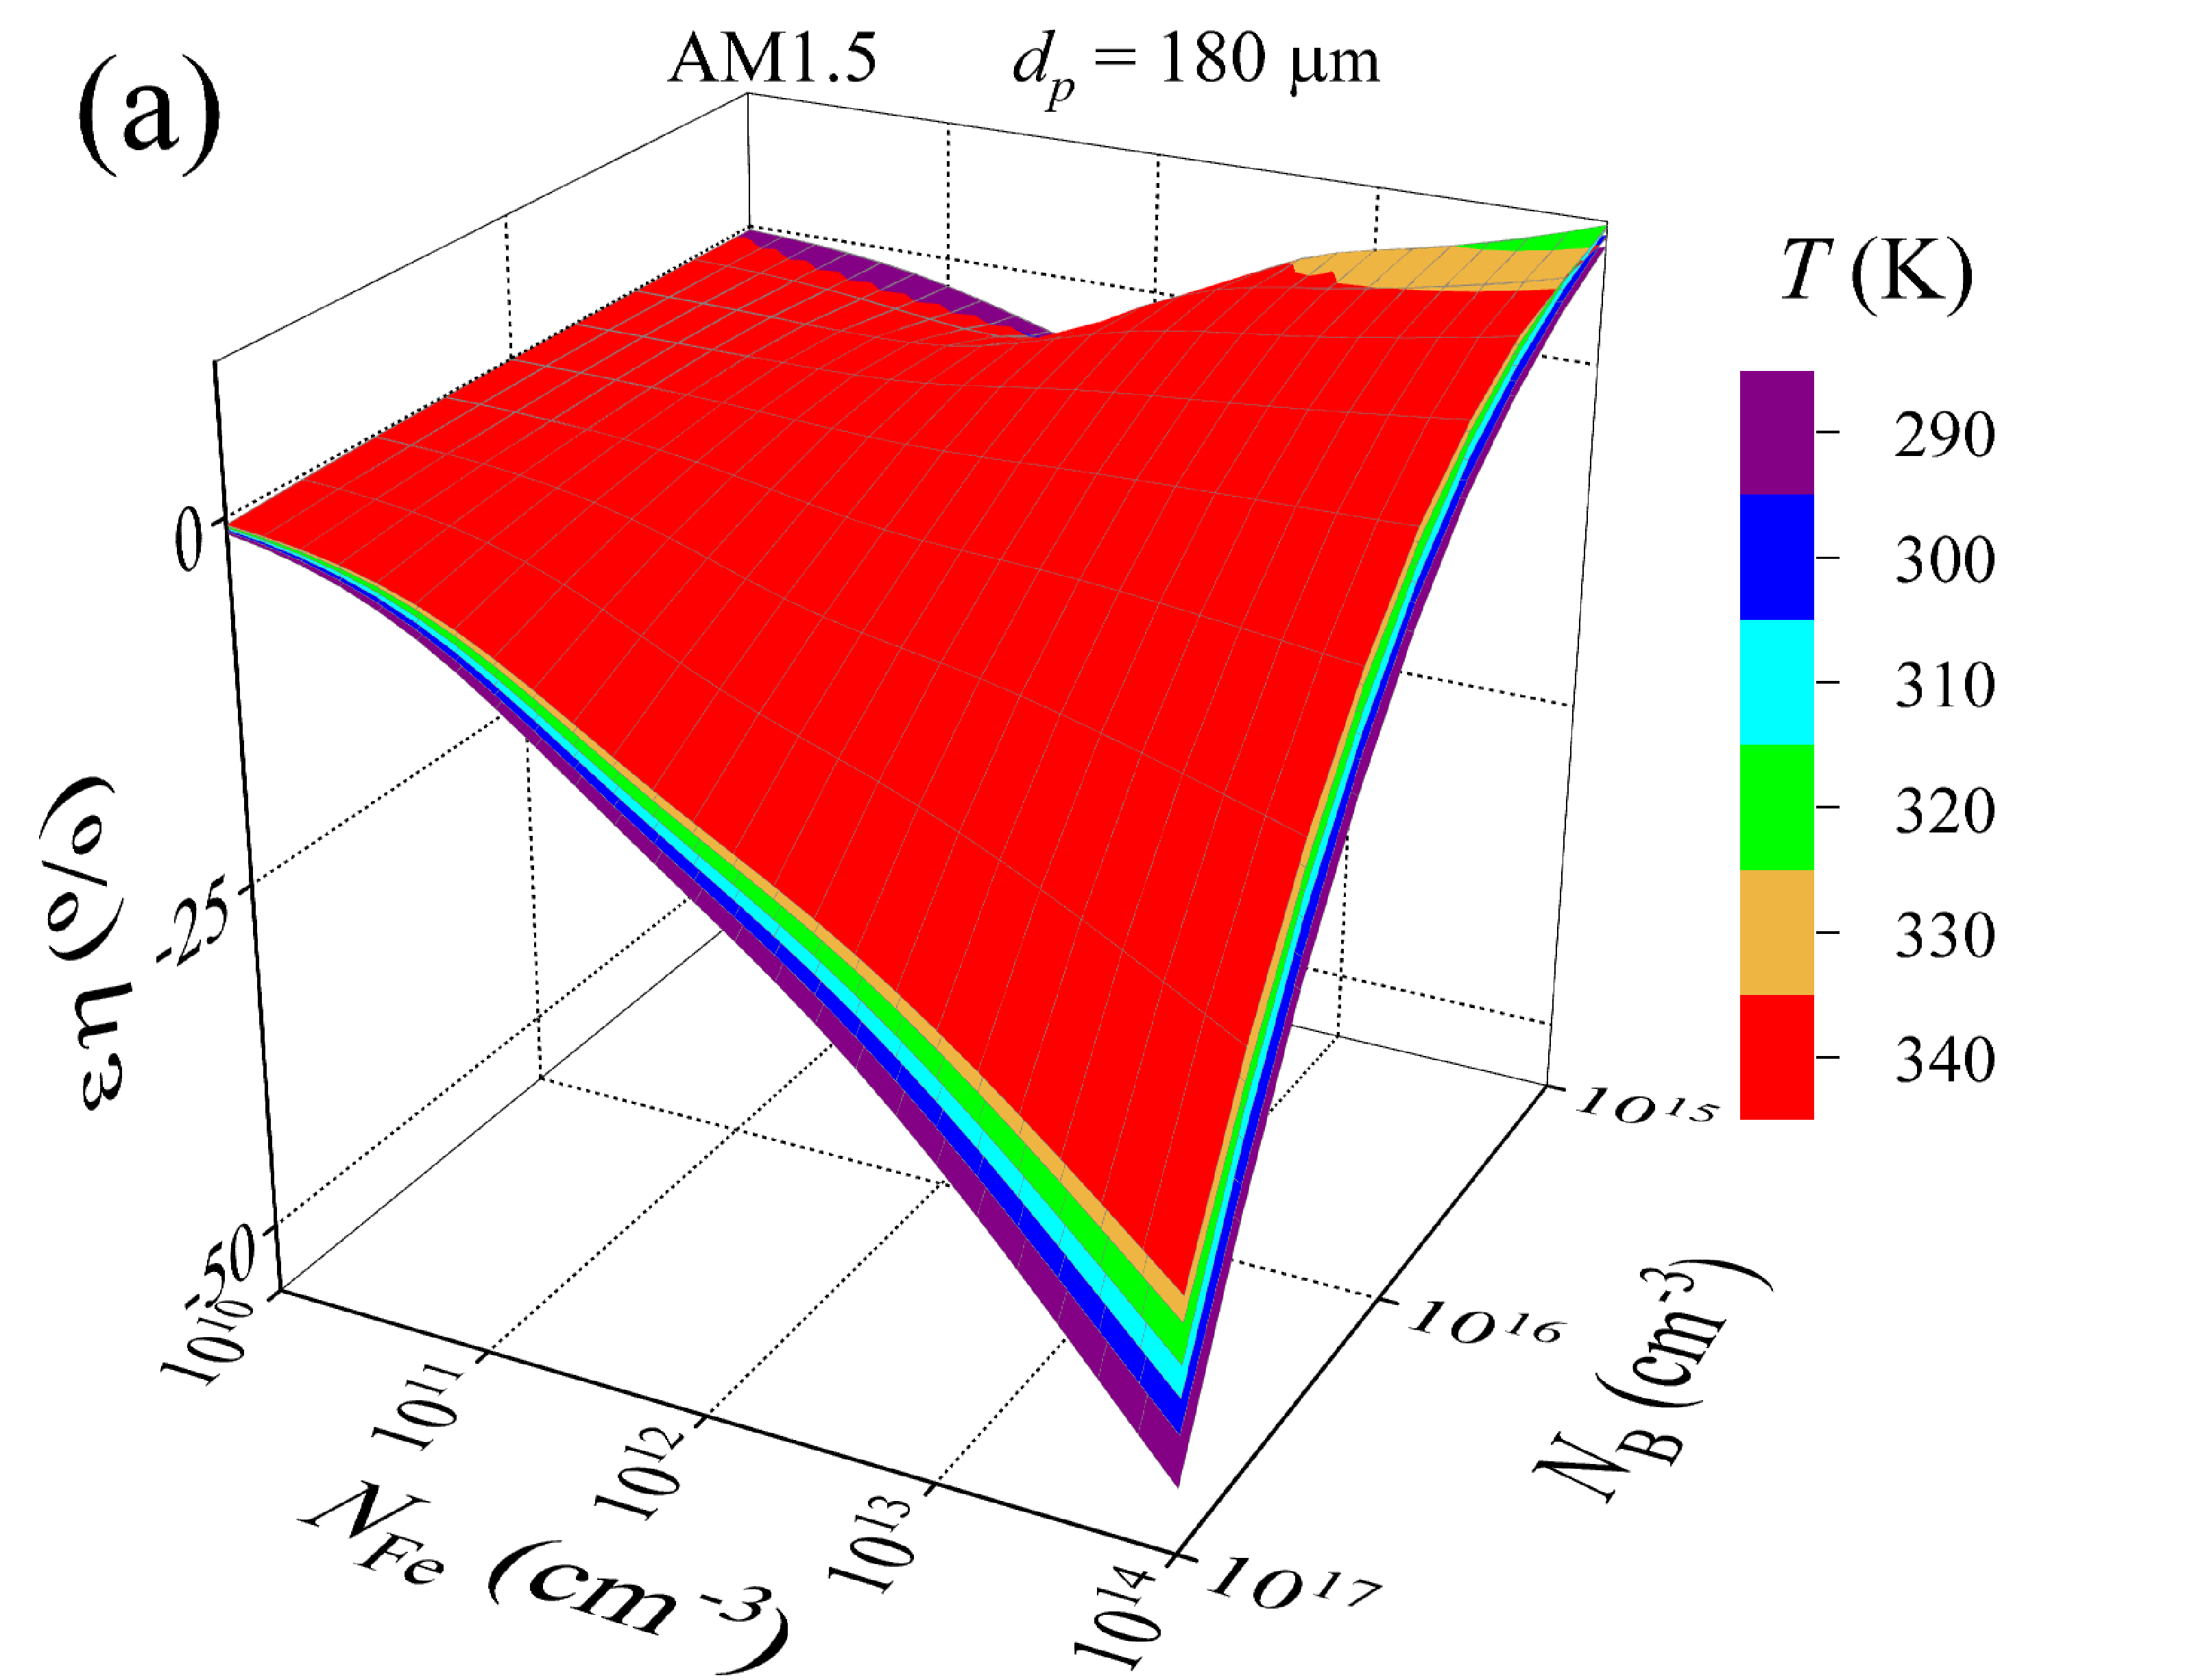
\includegraphics[width=0.34\linewidth]{Ris11.png}
     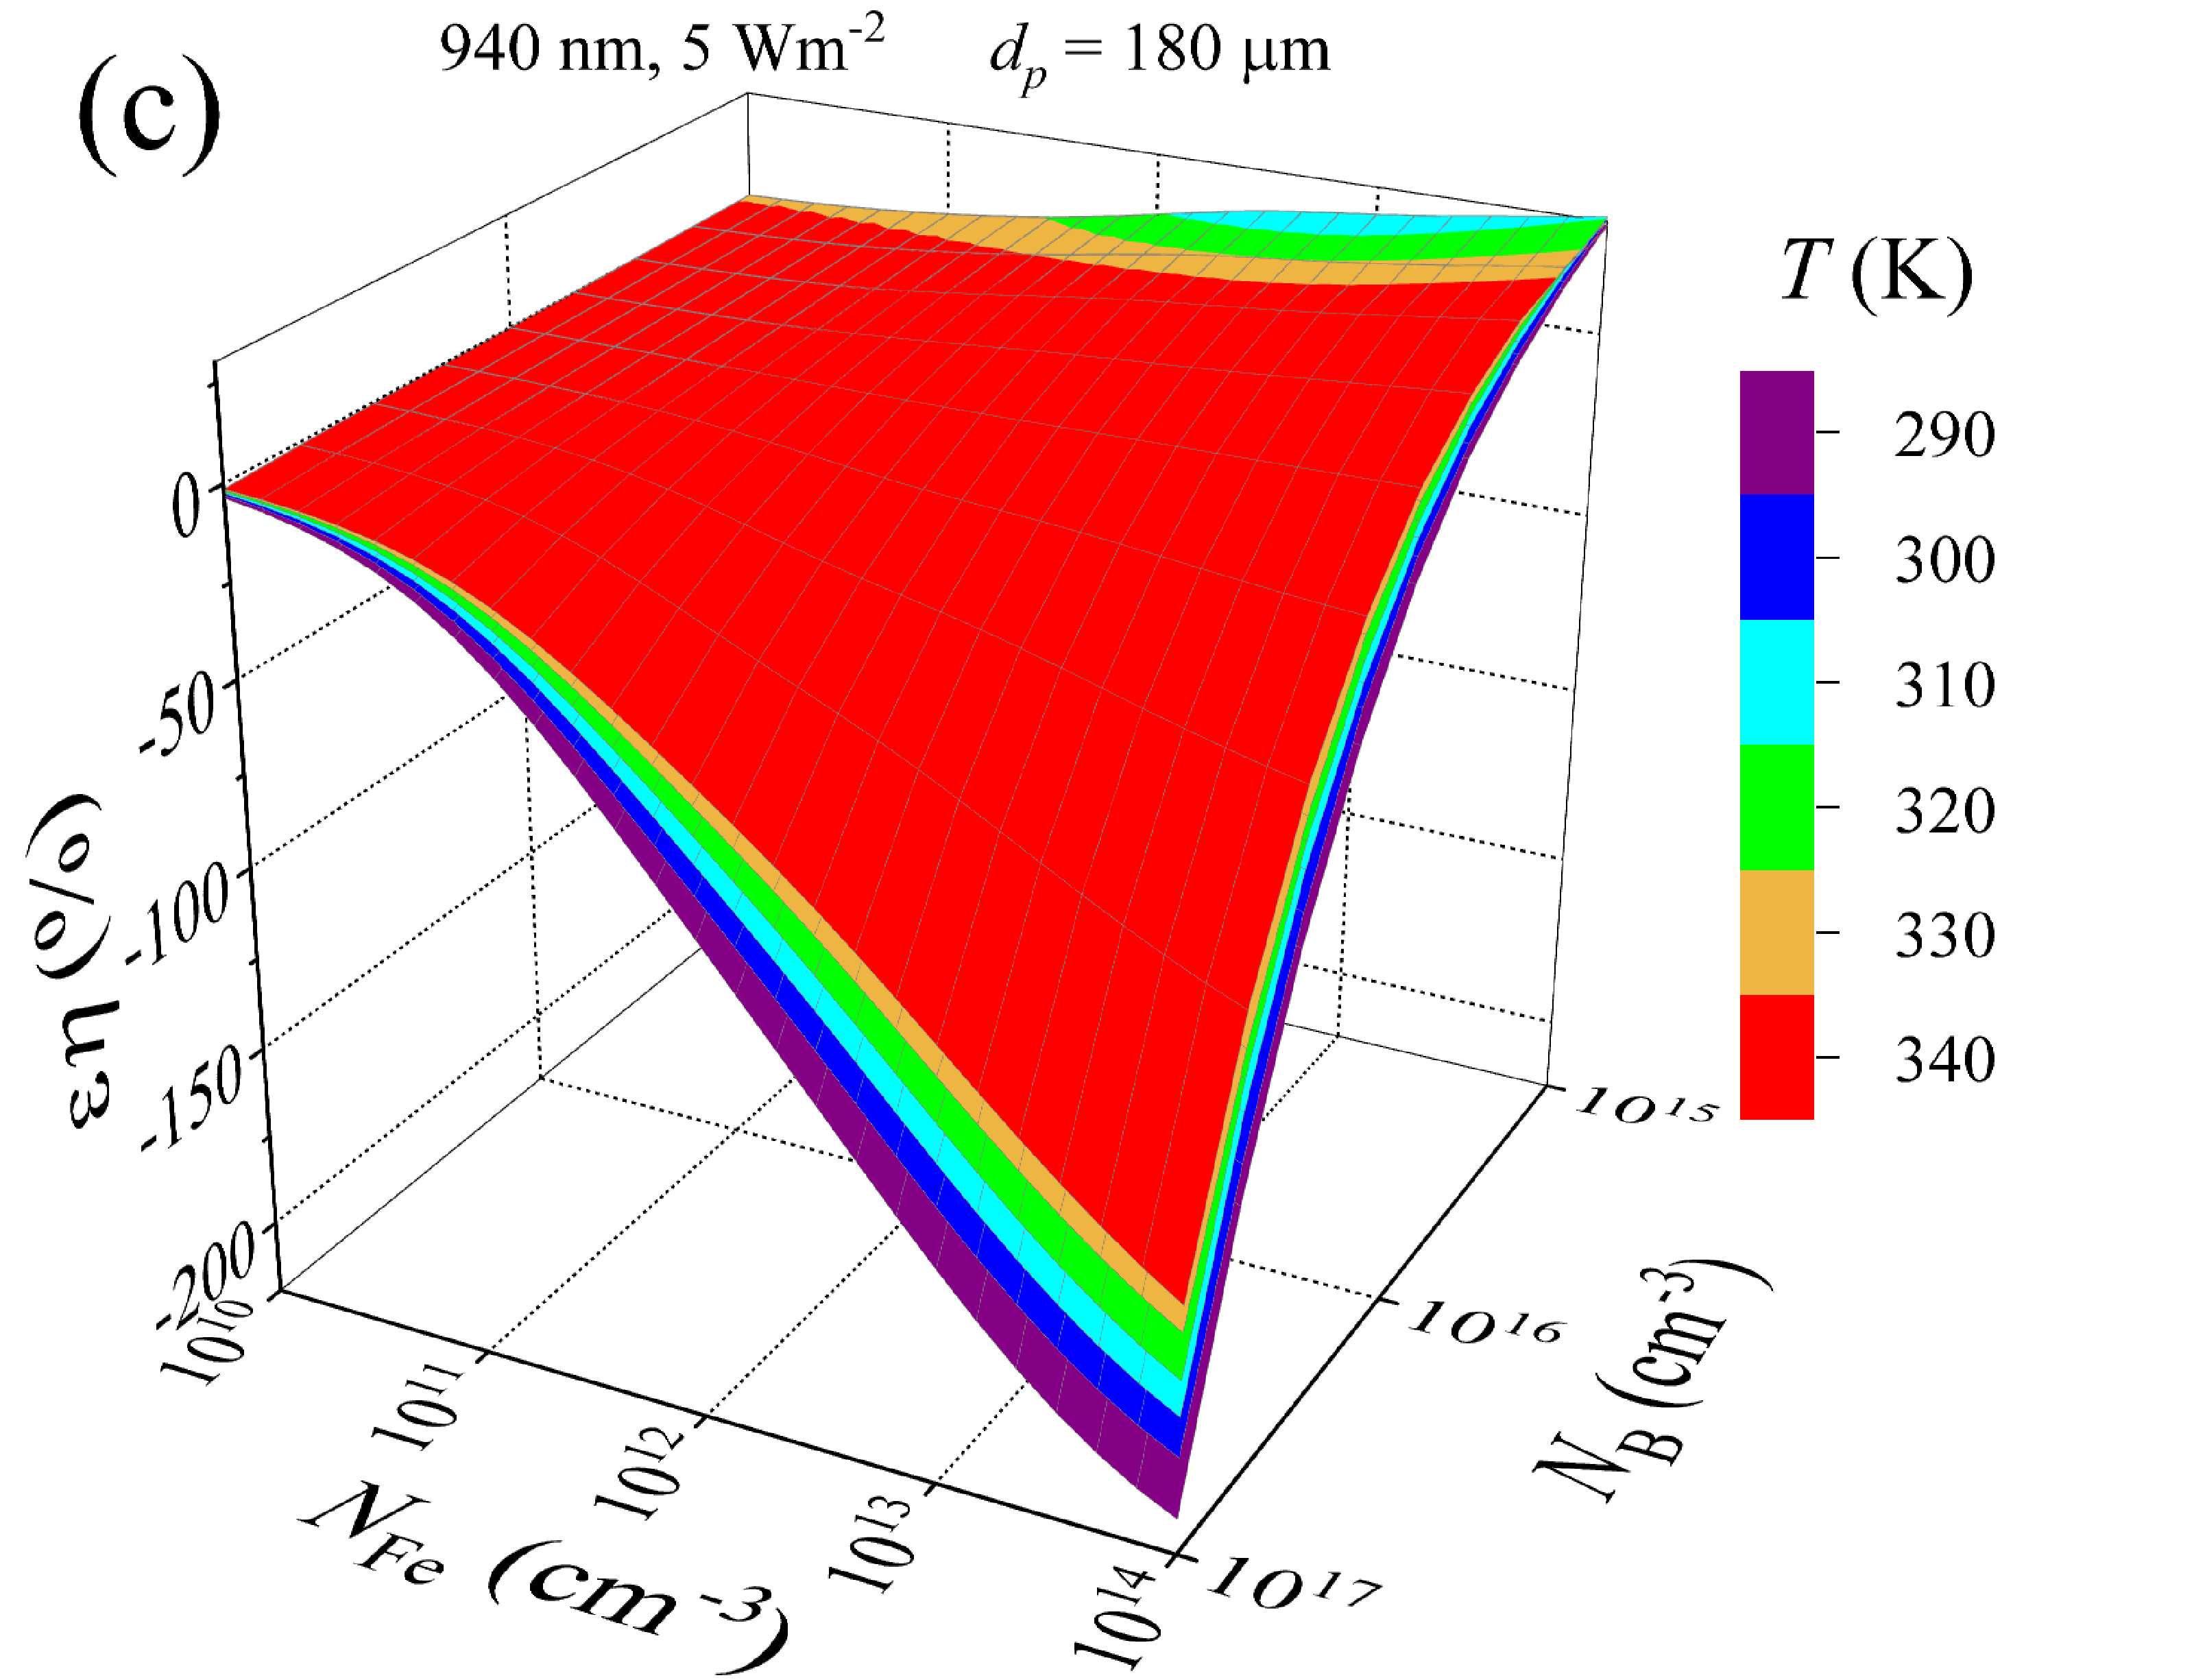
\includegraphics[width=0.34\linewidth]{Ris12.png}
     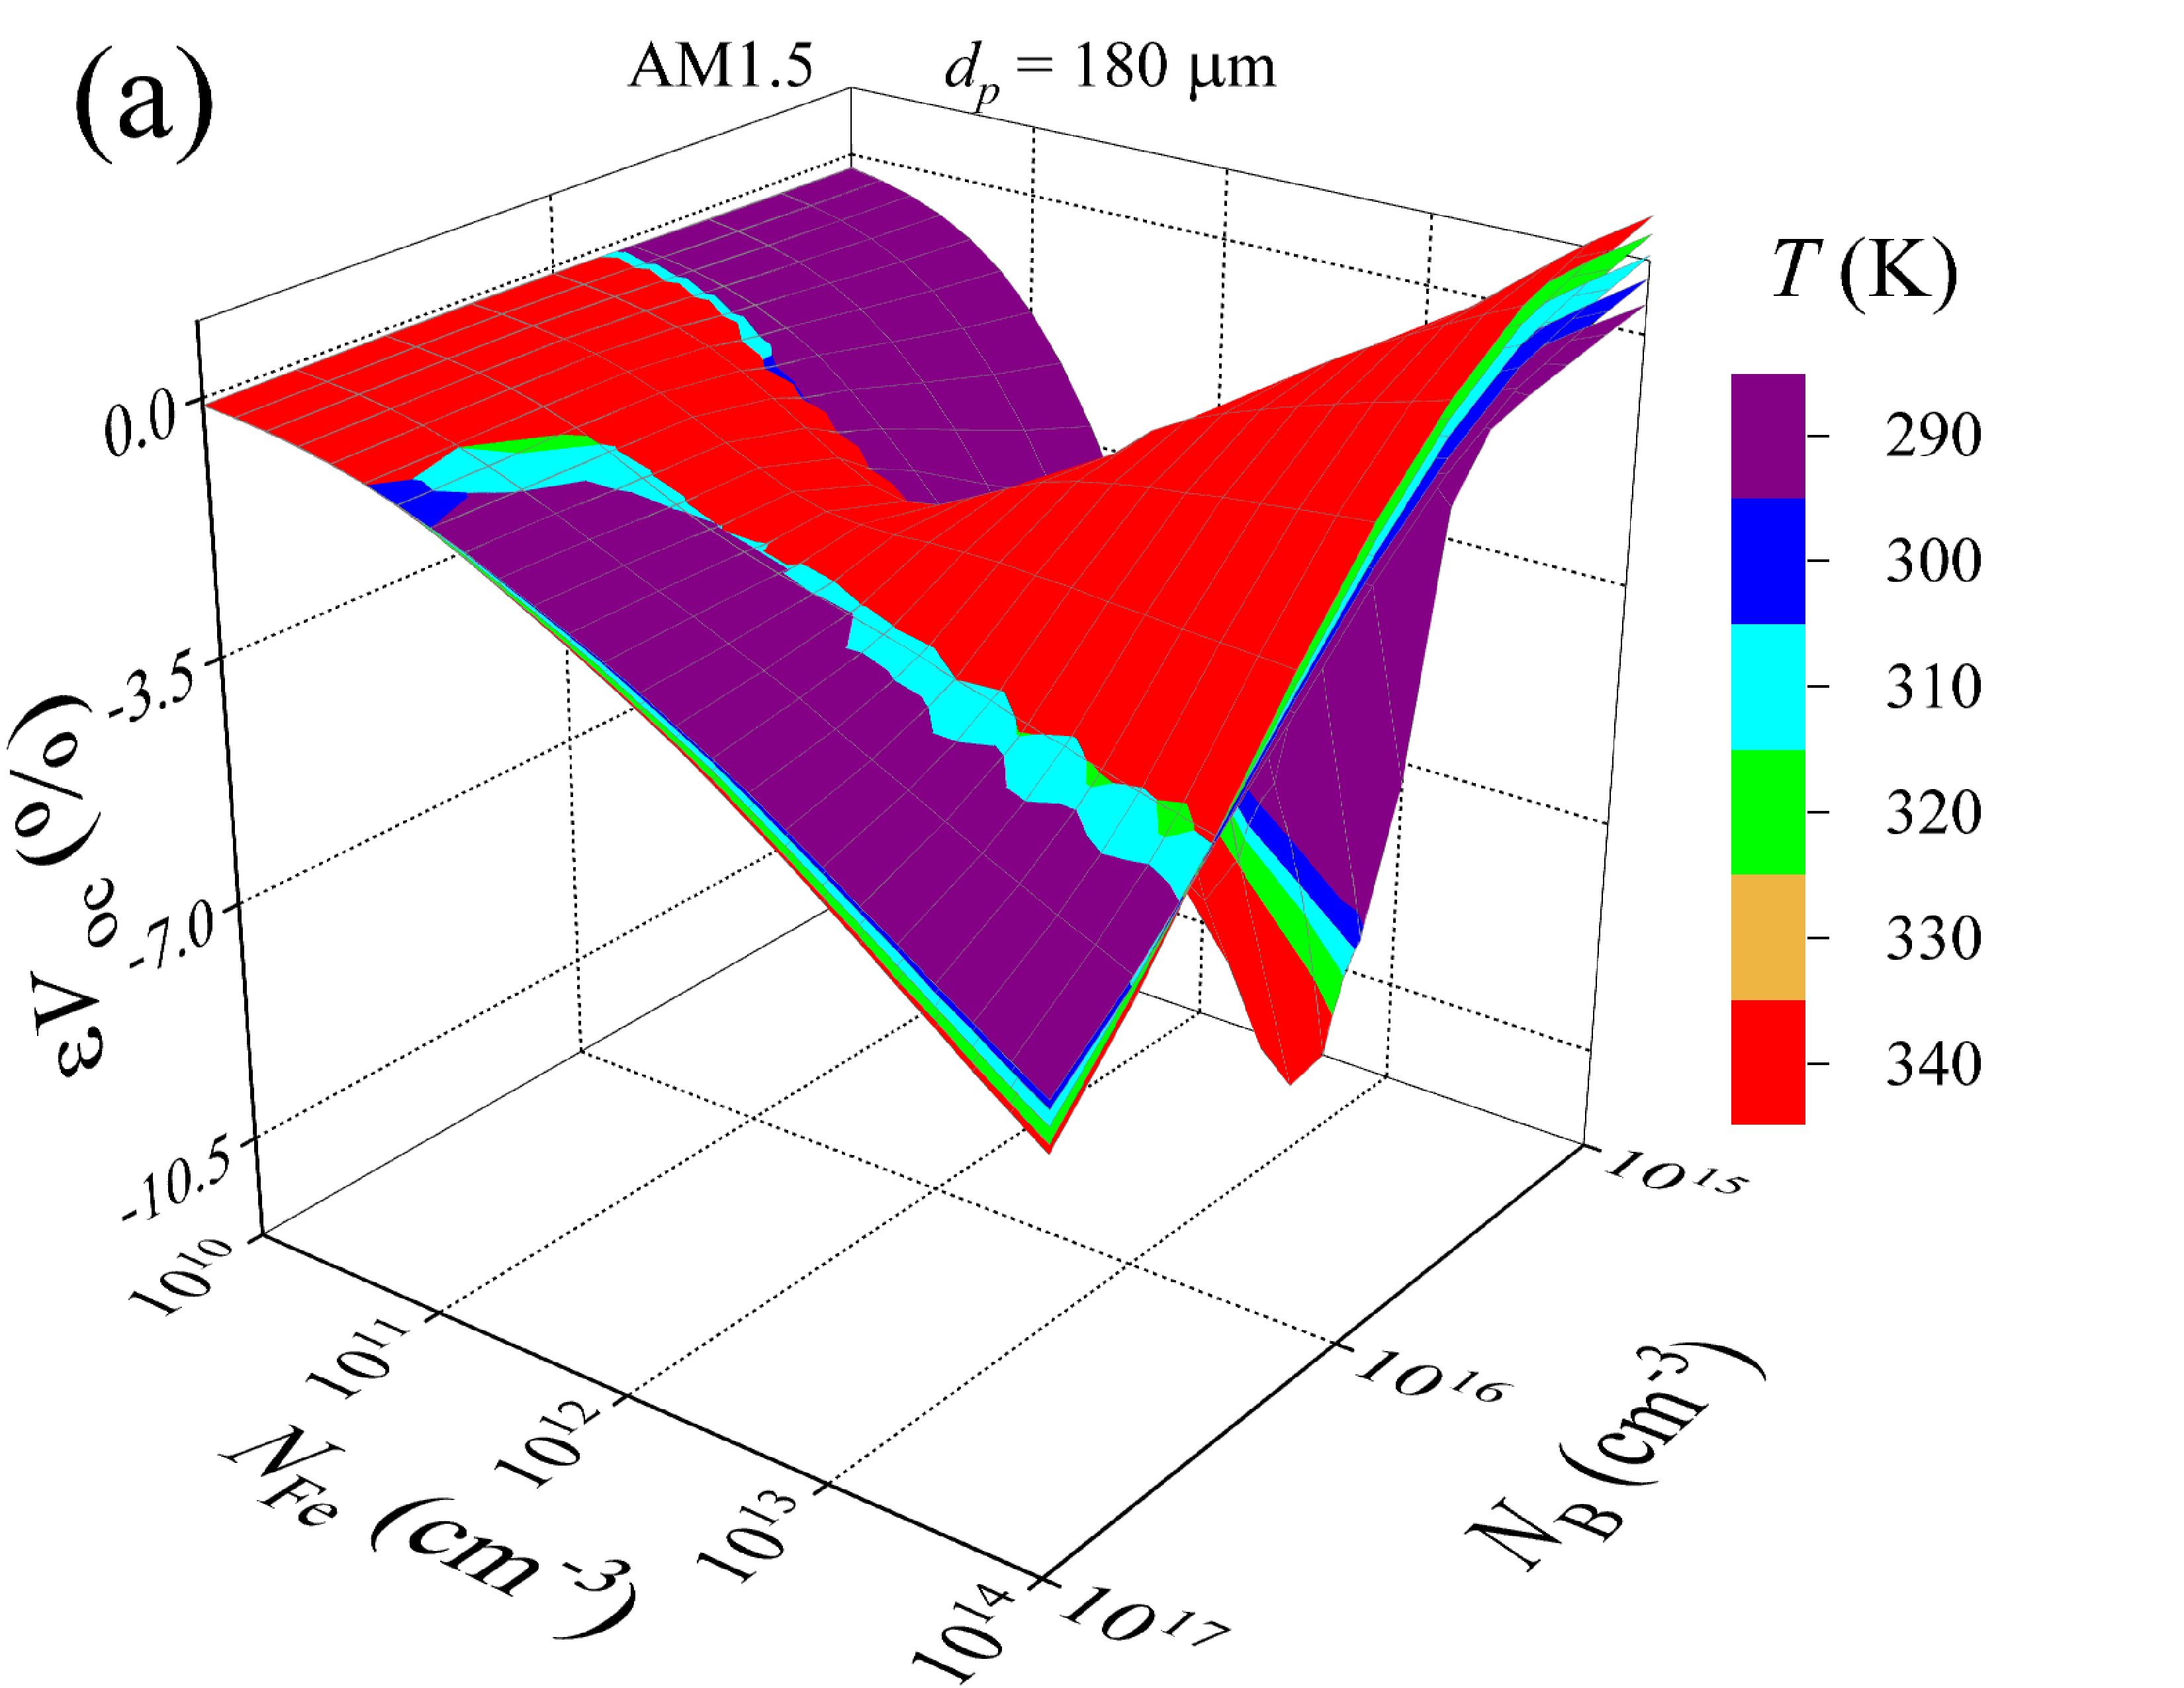
\includegraphics[width=0.34\linewidth]{Ris13.png}
     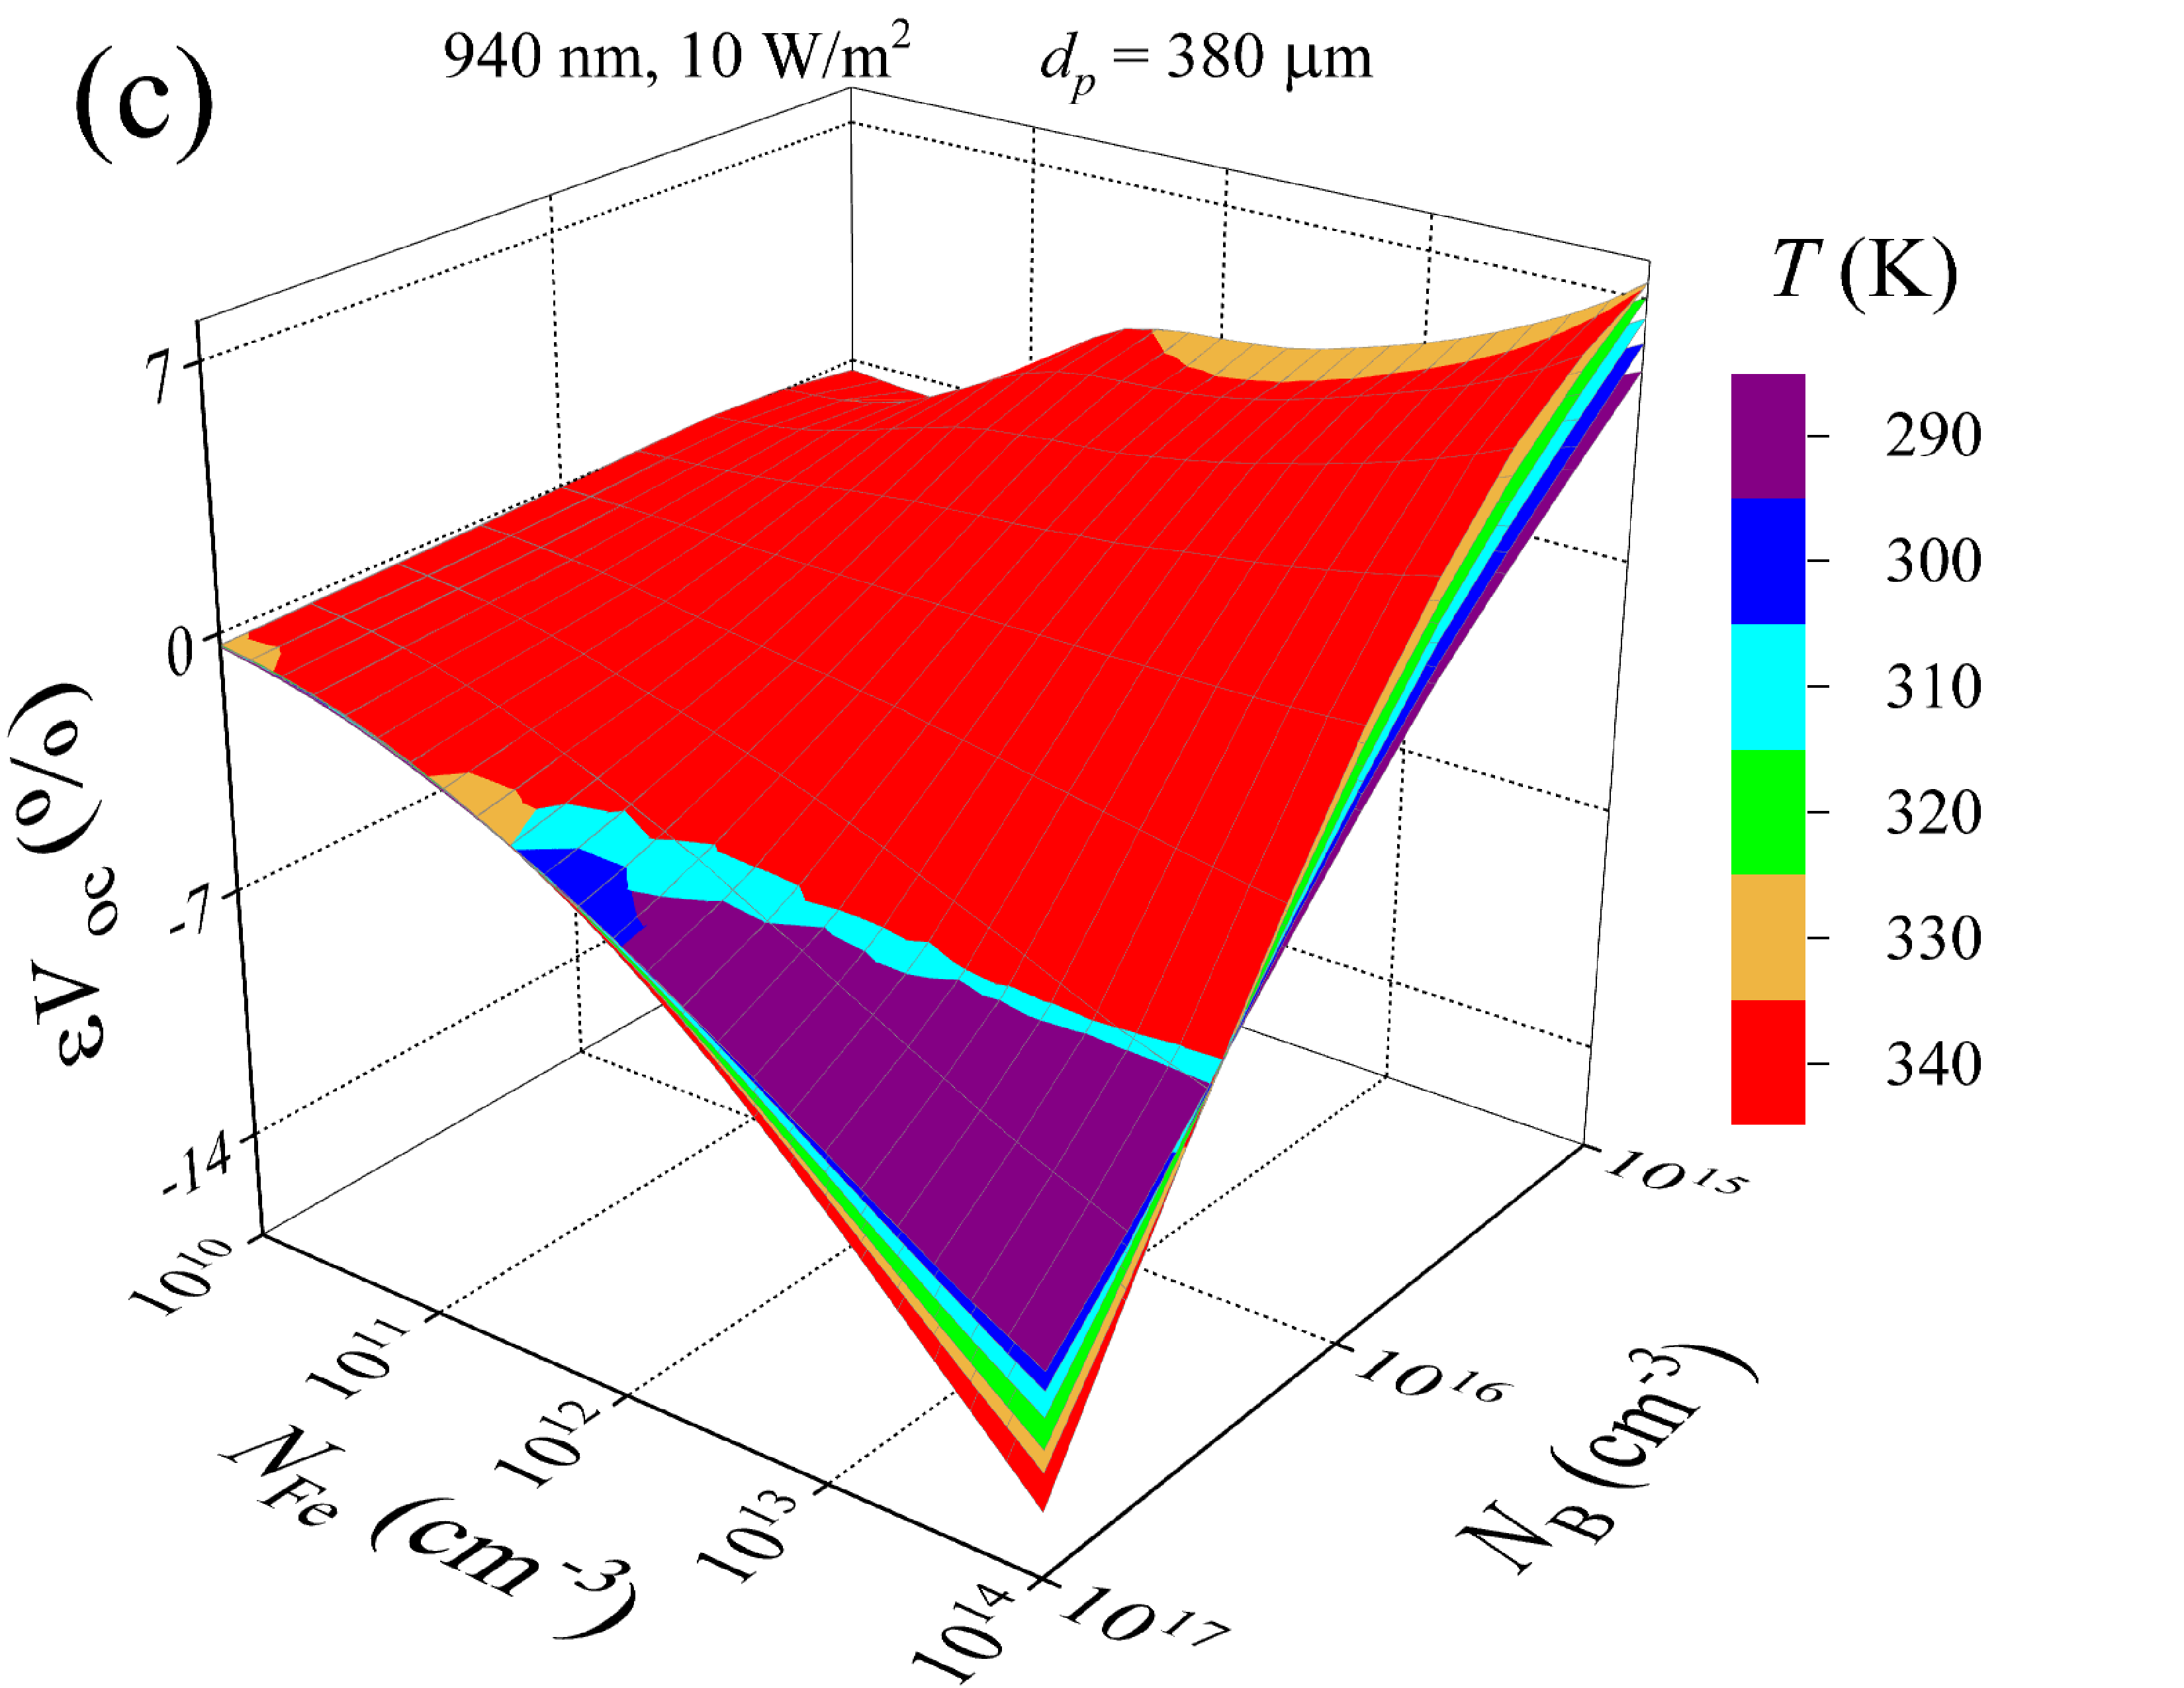
\includegraphics[width=0.34\linewidth]{Ris14.png}
     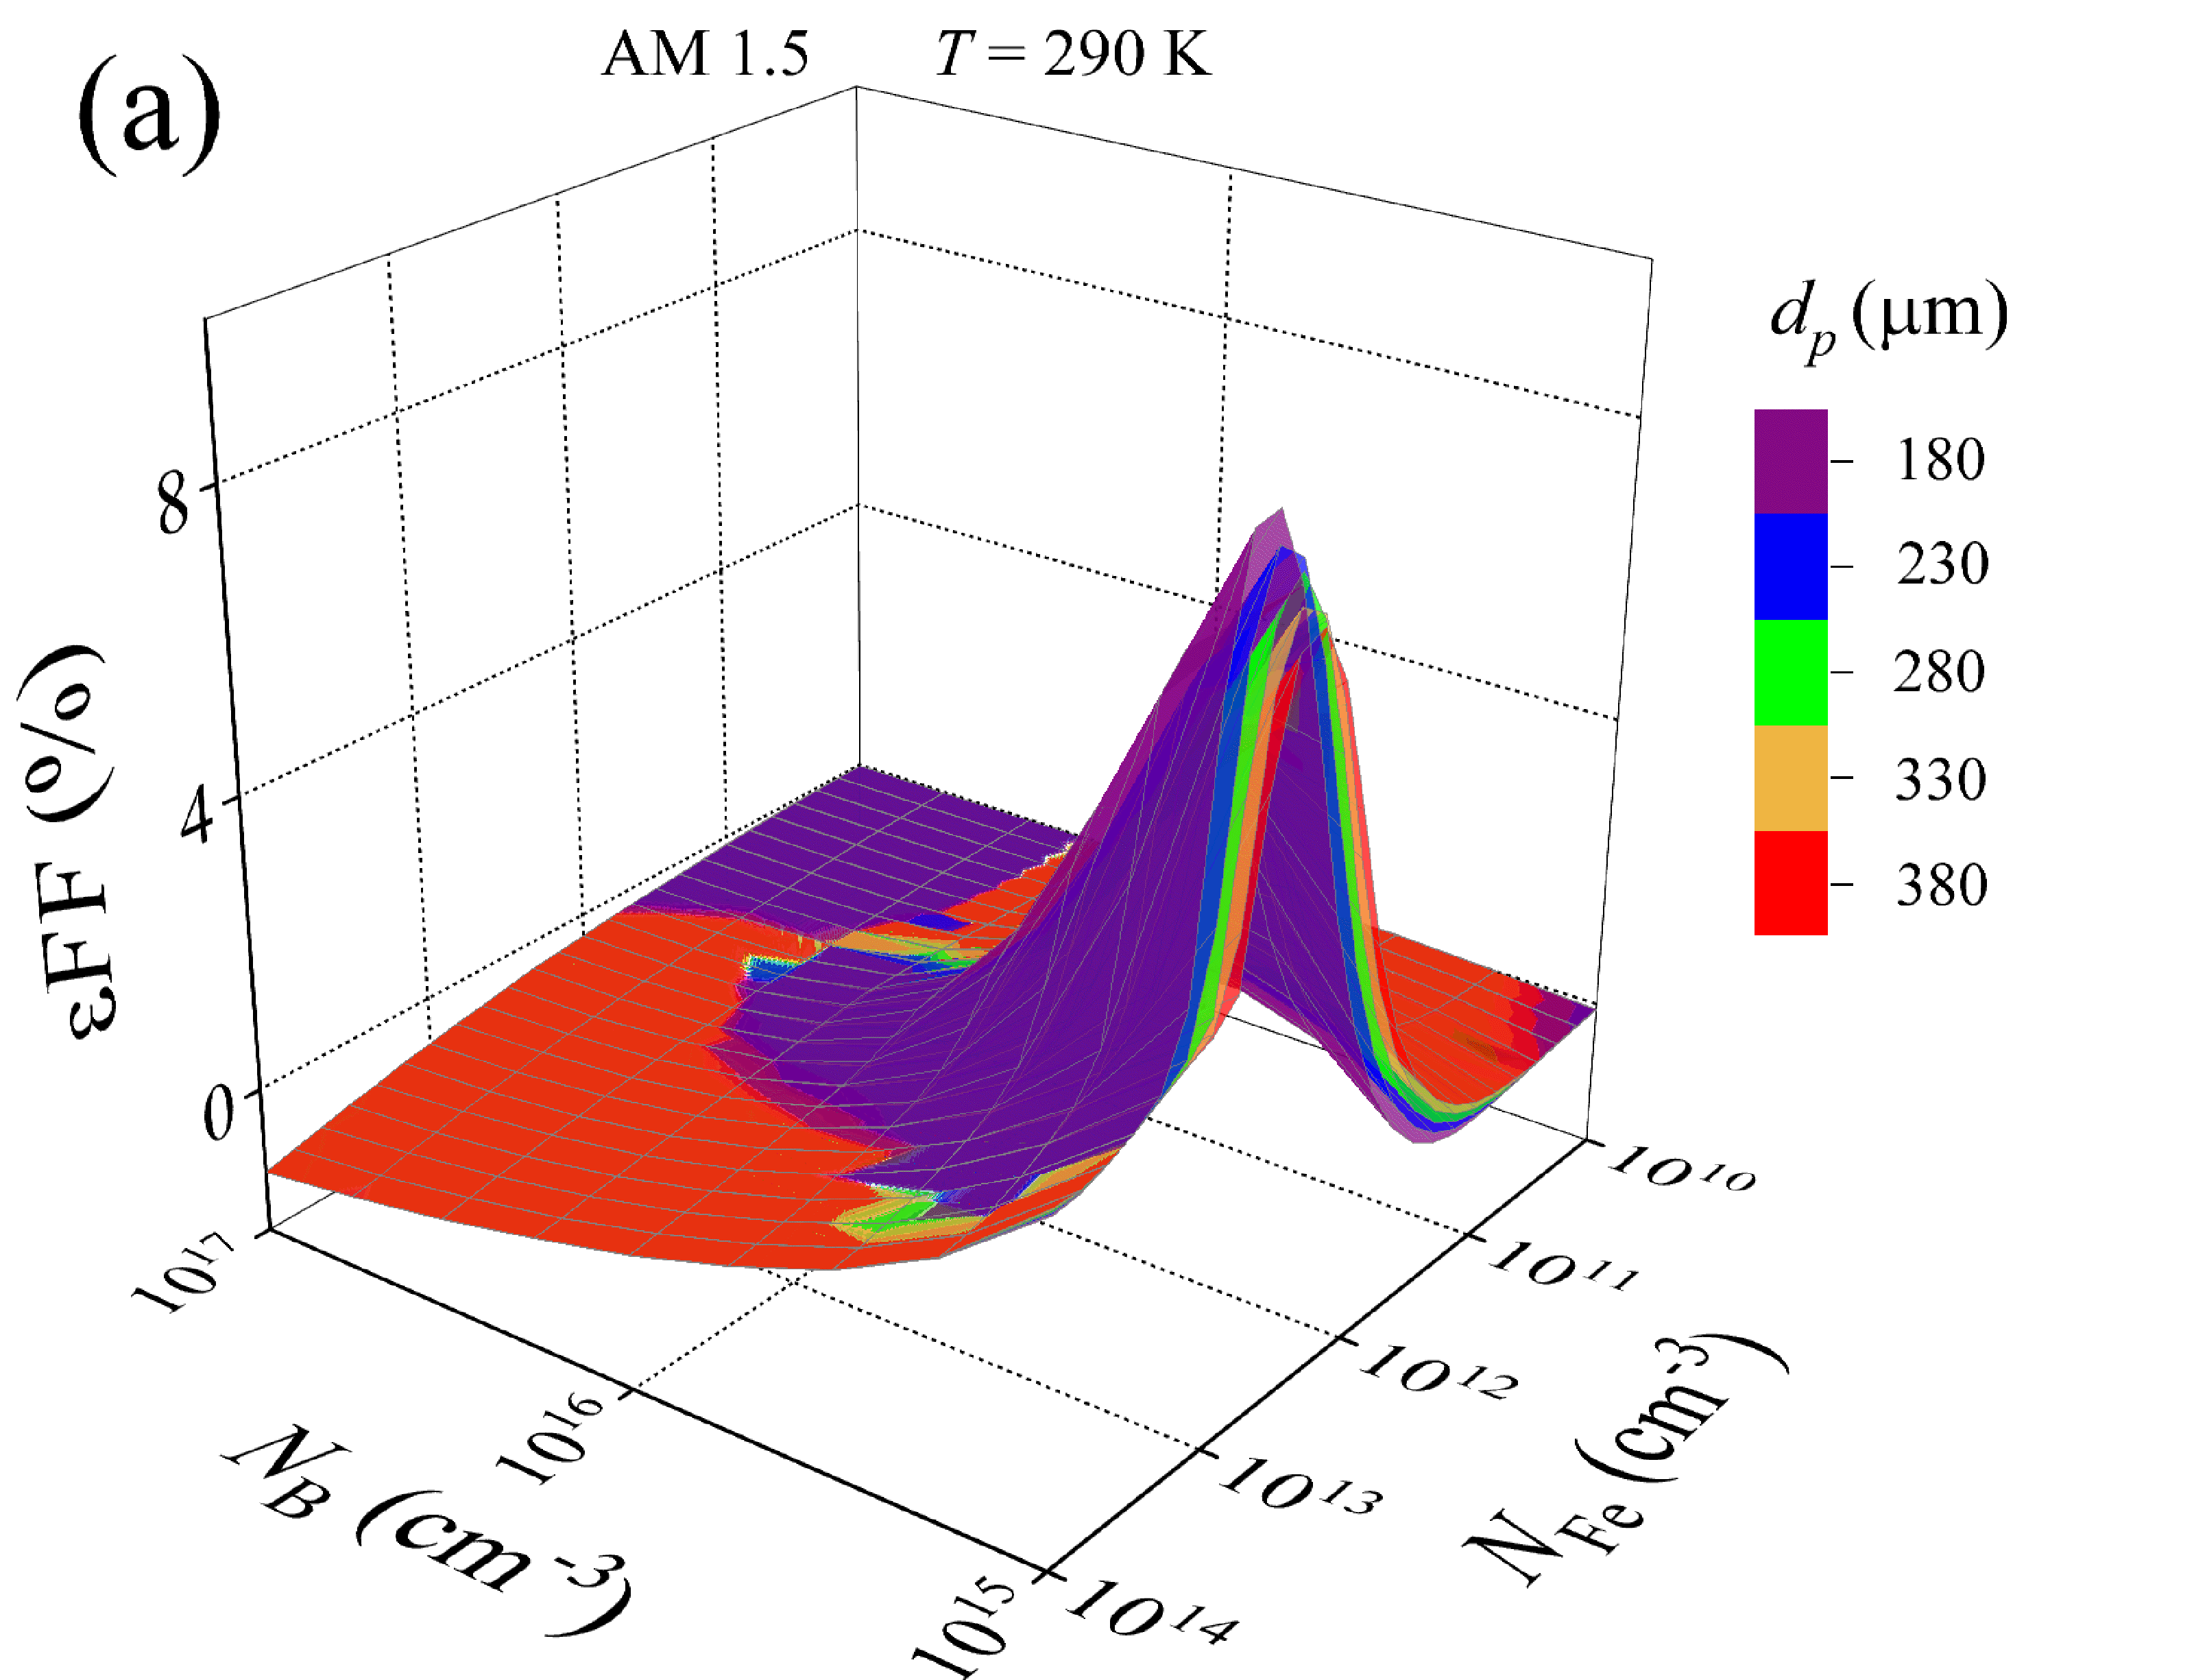
\includegraphics[width=0.34\linewidth]{Ris15.png}
     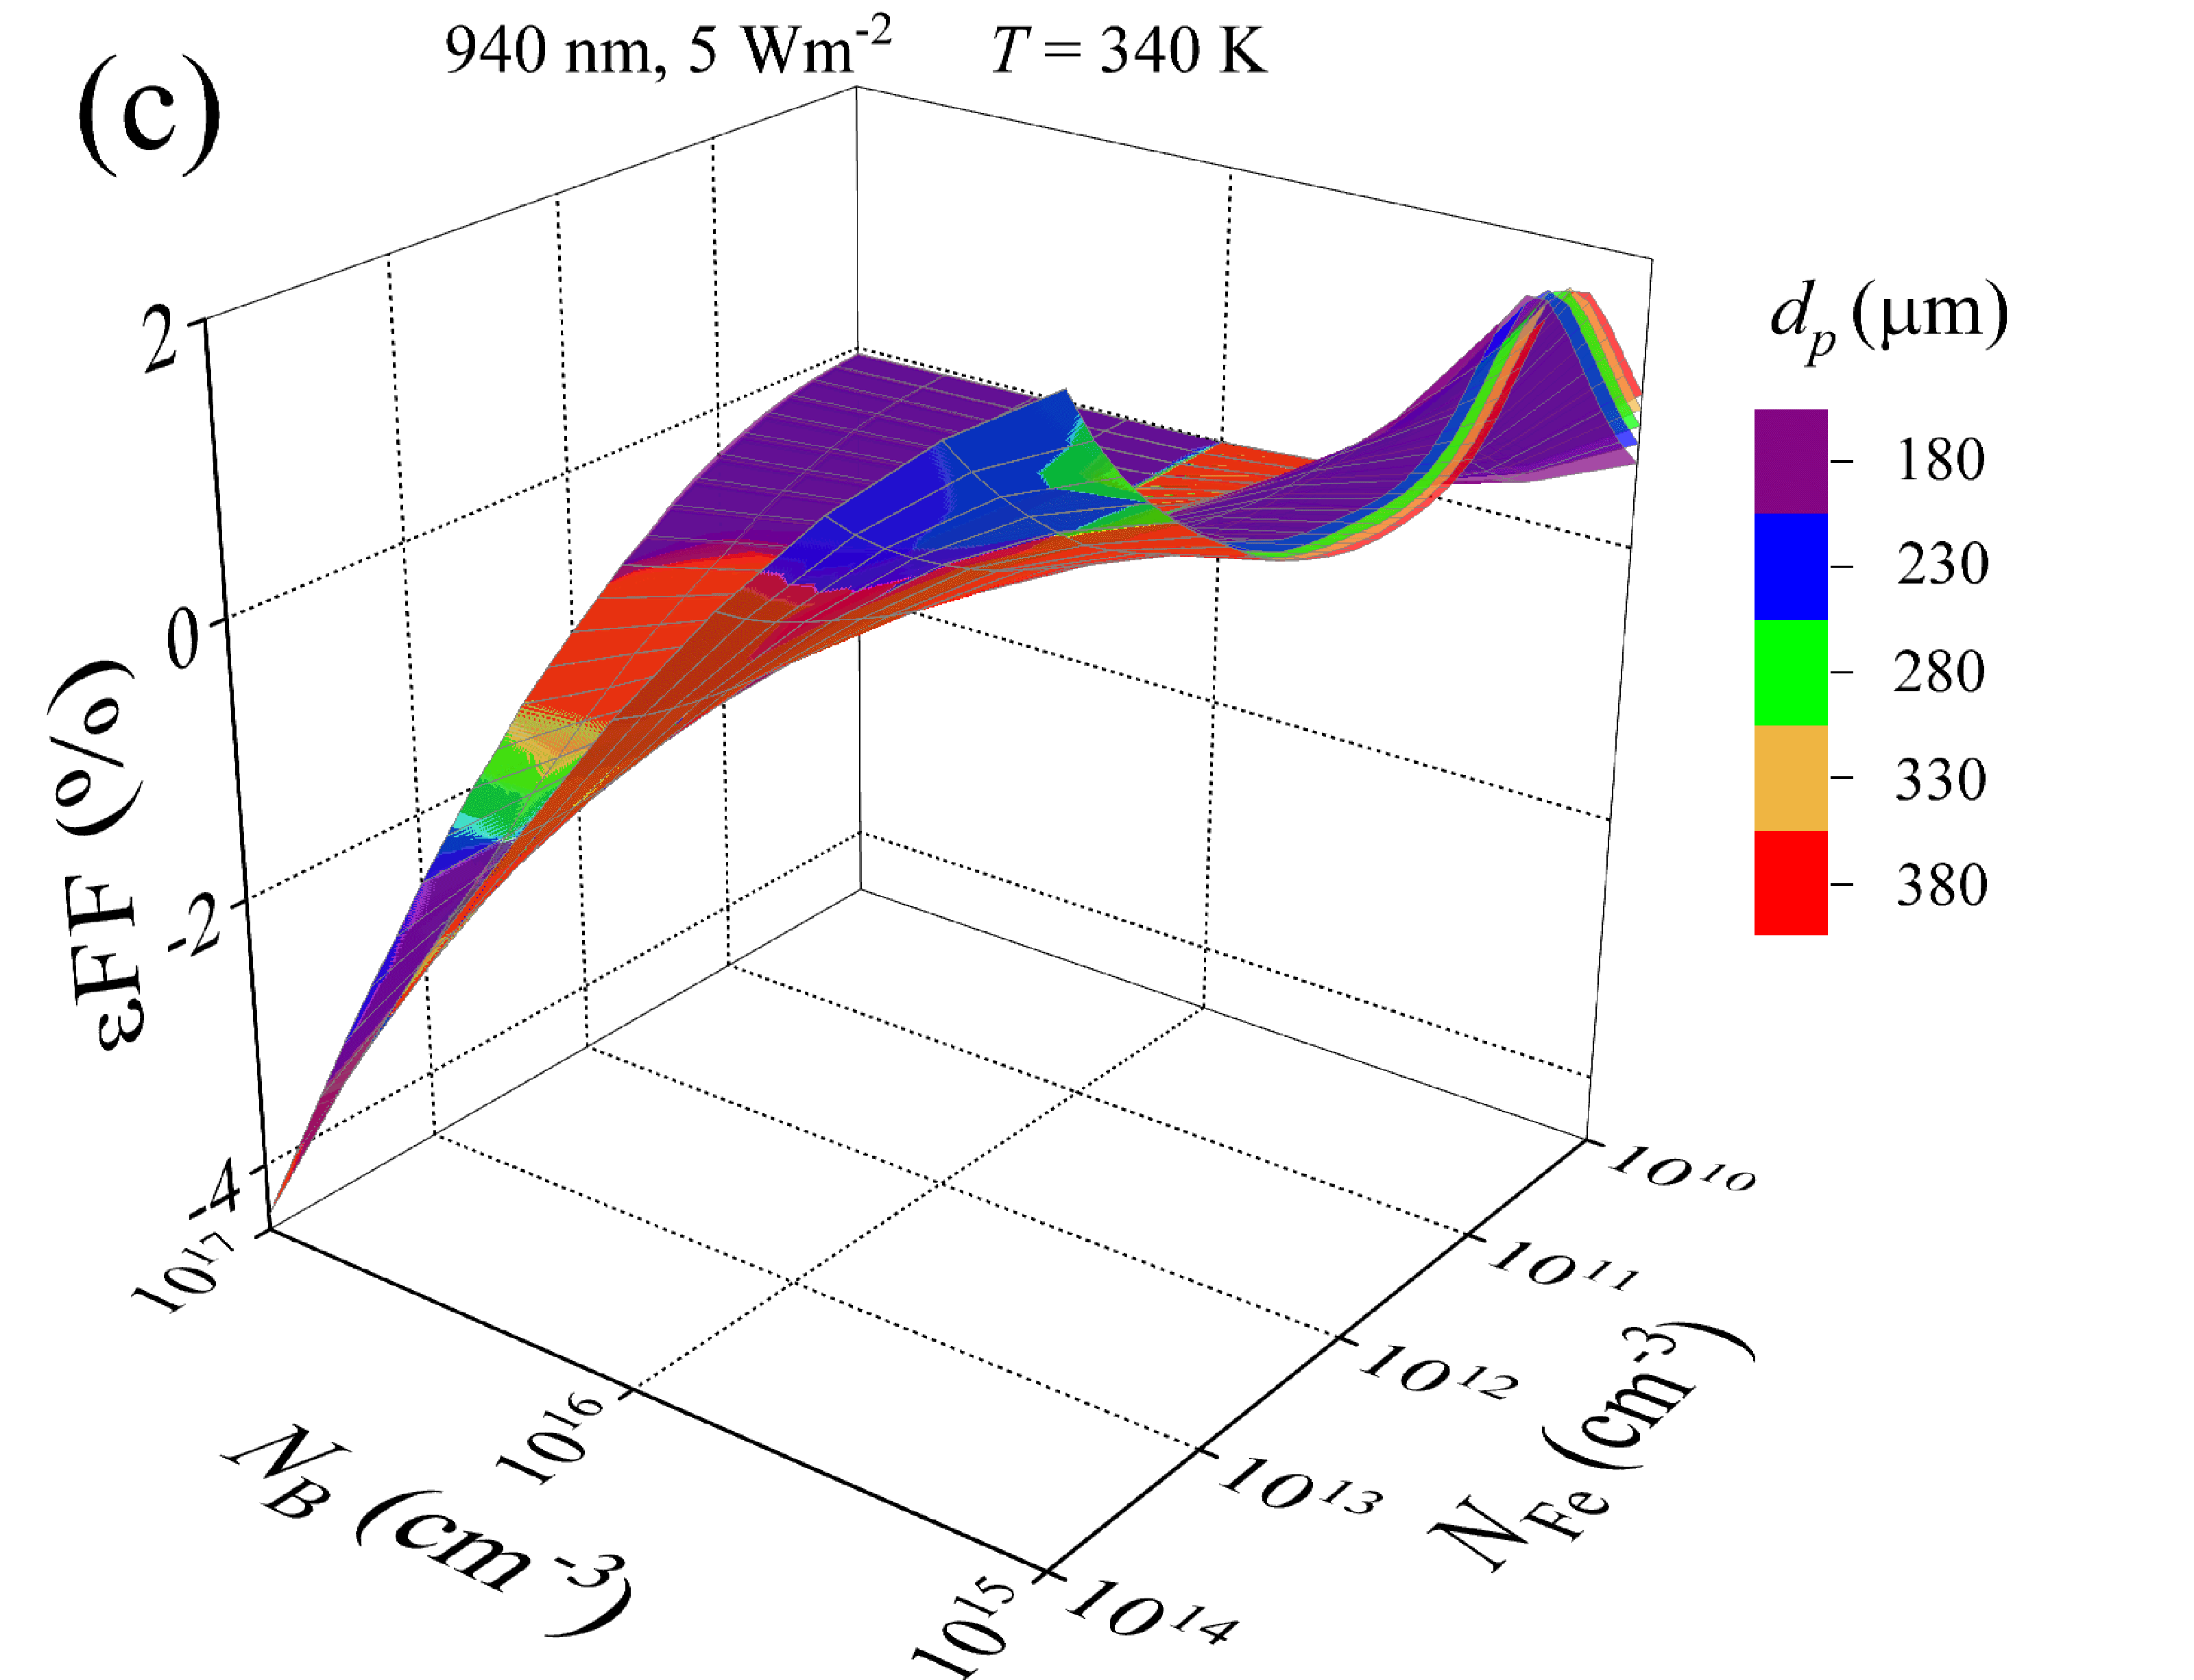
\includegraphics[width=0.34\linewidth]{Ris16.png}
	  \caption{Relative changes in solar cell efficiency (first row), open-circuit voltage (second row), fill factor (third row)
 caused by a complete dissociation of Fe$_i$B$_s$.
 The dependencies are shown for two cases:
 AM1.5 illumination (left column) and 940 nm monochromatic light (right column).
 The figures are taken from reference \cite{Olikh2025MSEB}.
}\label{fig1}
\end{figure}


This answer is incorporated in the text on page 16, last paragraph and page~17, first paragraph.




\vspace{1cm}
\noindent
\textcolor[rgb]{0.00,0.50,1.00}{\textbf{Comment~4.}}
\emph{Authors are suggested to provide more explanation behind failure of the particular model, infact, for the results obtained.}

\noindent
\textcolor[rgb]{0.51,0.00,0.00}{\textbf{Reply:}}

We thank the Reviewer for the valuable comment.
We fully agree that discussing potential reasons for the discrepancies in model performance is essential.
In fact, our response to the previous comment already addresses part of this issue.
Upon further examination of other cases, we note the following:



Increasing the number of descriptors while keeping the sample size constant leads
to higher sparsity in the data space due to increased dimensionality,
which in turn makes it more difficult for the model to generalize.
In such cases, the model may also learn spurious correlations that do not generalize to test data ---
a risk that is particularly pronounced in deep neural networks and  deep tree-based ensemble methods.
Moreover, a larger number of features results in more model parameters, increasing the risk of overfitting.
These factors can collectively lead to a reduction in prediction accuracy.
In our opinion, for A$^\mathrm{AM1.5}$ models, both the positive effects achieved by increasing the number of descriptors
(enhancing overall information variance and reducing ambiguity between the target variable and the input features) were dominant.
However, for A$^\mathrm{940}$ models where this ambiguity was already low,
the negative effects described above outweighed the benefits,
which explains why prediction accuracy did not improve when using an expanded feature set.

Another effect that may arise when increasing the number of features is multicollinearity.
It occurs when new features are highly correlated with existing ones and can lead to instability in model estimates.
However, in our case, it is unlikely that multicollinearity among the photovoltaic parameters
(incidentally, their correlation is significantly higher in the 940 nm case than in the AM1.5 case — see Fig.~S1)
affects prediction accuracy.
First, all algorithms used are sufficiently robust to multicollinearity.
Second, a standard method for mitigating multicollinearity is PCA.
Despite previous successes in applying principal component analysis to various
photovoltaics-related machine learning tasks \cite{Gao2020,Fadhel2019,David2021,Liu2022,AbdullahVetter2025} ---
and the presence of favorable conditions for its use in our case,
such as the high correlation between changes in photoelectric parameters caused by FeB pair dissociation ---
applying PCA as a data pre-processing step for evaluating iron impurity concentration did not improve the maximum prediction accuracy in most cases.
One likely reason is that PCA preserves the overall variance in the data
but does not account for the specific relationships between individual features and the target variable.
For instance, some photovoltaic parameters may be more informative for predicting low iron concentrations,
while others may be more relevant for high concentrations.
For instance, $\varepsilon F\!F$) are shown \cite{Olikh2025MSEB} to be most pronounced at low iron concentrations, unlike other PVPs.
When these components are merged through PCA transformation, such distinctions may be lost, leading to reduced accuracy.
Another possible reason is that principal components ---
being linear combinations of original features --- do not support localized decision splits
(i.e., those based on individual feature thresholds), which are particularly effective in tree-based models.

When comparing the effectiveness of different algorithms, several points are worth noting.
The poorest performance observed with SVR is likely due to its limited ability
to model complex nonlinear relationships ---
such as those that apparently exist between iron concentration and variations in photoelectric parameters.
In contrast, the superior performance of the XGB and DNN models is attributable to
their ability to effectively capture nonlinear patterns, which in our case become more prominent with increasing descriptor dimensionality.
Specifically, XGB performs best in relatively simpler scenarios, such as those involving 940 nm illumination
(see Figs.~7i-7l, 9i-9l).
This is because XGB requires less training data than DNN
(12,000 examples are sufficient, though this is not a particularly large amount for a neural network),
handles high-quality structured data well (simulated data are noise-free),
and is more resilient to the influence of correlated features.
At the same time, DNNs are more powerful tools for nonlinear modeling,
capable of uncovering hidden structures in the data.
This enables them to achieve better results on more complex tasks ---
such as the transition to A$^\mathrm{AM1.5}$-models with high-dimensional features
(see Figs.~7m-p, 9m-9p).
As shown by the results in Subsection~3.4, successful prediction within the
$N_\mathrm{B}$--altered also requires accounting for higher-order relationships,
which explains why DNN models achieved the best performance (Figs.~11e-11l).
Regarding the RF and GB algorithms, as indicated in Tables~1 and 2,
they tend to perform best only on less complex data
(i.e., small sets of descriptors), where more powerful models are at higher risk of overfitting.

Reply has been incorporated into revised manuscript as Subsection~3.5.

\vspace{1cm}
\noindent
\textcolor[rgb]{0.00,0.50,1.00}{\textbf{Comment~5.}}
\emph{What can be done to further increase the accuracy of these models?}

\noindent
\textcolor[rgb]{0.51,0.00,0.00}{\textbf{Reply:}}

При розгляді можливих шляхів збільшення accuracy of models насамперед потрібно врахувати що саме вже було зроблено в цьому напрямі.
А саме, були проведені нормалізація даних, використані різні набори дескрипторів, 
розглянуто доцільність зменшення кореляції ознак завдяки PCA, 
проведено налаштування основних параметрів моделей  (див. Table S1-S5, Fig. S2) з використанням Bayesian Optimization (пакет Optuna),
використано крос-валідацію.

Серед того, що лишилося і виглядає виправданим можемо виділити наступне:
1) збільшення тренувального набору, насамперед за рахунок використання більшого числа значень концентрації бору в базі:
найбільш очевидний шлях, що відображає головну особливість машинного навчання, а саме потребу у щонайбільшому об'ємі даних;
2) викостати існуючі дескриптори для створення нових, які будуть більш однозначно та просто пов'язані з концентрацією заліза;
зрозуміло, що це не можуть бути лінійні комбінації, що застосовуються під час РСА, і для їх створення необхідно орієнтуватися насамперед на фізичні процеси;
3) долучити нові ознаки; при цьому бажано, щоб для їхнього отримання не були потрібні додаткові вимірювання, так як подібні ускладнення суттєво знижують привабливість
запропонованого методу; наприклад, довжина дифузії неосновних носіїв могла б бути чудовим дескриптором, проте нам невідомі методи, які дозволяють її визначити на основі вимірювання однієї (двох)
вольт-амперних характеристик; найбільш очевидним цьому напрямі було б використання у ролі додаткових ознак напруги Vmp та струму Imp, які відповідають максимальній вихідній потужності, 
хоча, звичайно, їх не можна назвати незалежними від АА, Шв, ИМ.

Окремо можна виділити шляхи підвищення якості тренувального набору завдяки наближення моделі, яка використовуються під час моделювання до реальності.
Наприклад, замість SCAPS використати для створення labeled datasets 3D-simulators (e.g., Synopsys Sentaurus TCAD, Silvaco ATLAS TCAD чи Solcore) та врахувати
наявність інших домішок, наприклад найбільш типових для Cz-Si кисню та вуглецю.

Інший шлях досягнення збільшення точності прогнозів полягає у зміні стратегії створення моделі.
Наприклад, можна відмовитися від підготовки універсальної точки зору застосовності до різних сонячних елементів модель і зосередитися на сонячних елементах з конкретною будовою
(певні значення Вз та Т). 



\textcolor[rgb]{1.00,0.07,0.00}{
\hl{}}

The accuracy of the models could be further improved by:
\begin{itemize}
    \item \textbf{expanding the training data set}: simulating a broader and denser range of device parameters 
    (e.g., more values for doping, thickness, temperature, and iron concentration) would provide 
    the models with more comprehensive training examples and improve generalization;
    \item \textbf{model optimization}: further tuning of model hyperparameters, or employing more sophisticated ensemble or deep learning architectures, 
    could enhance predictive performance;
    \item \textbf{enhancing the physical realism of simulations}: incorporating even more detailed or advanced physical models in SCAPS, 
    such as additional defect types, surface effects, or more accurate material parameters.
\end{itemize}


%Прогнозувати не конкретне значення, а розподіл:
%
%    Використовують байєсівські моделі, мішані моделі, або нейронні мережі з варіаційним виведенням.
%
%Прогнозувати середнє або медіану:
%
%    Це те, що робить, наприклад, регресія — дає очікуване значення E[y∣x]E[y∣x], навіть якщо реальність складніша.
%
%Моделювання з шумом або латентними змінними:
%
%    Залучають приховані фактори або генеративні моделі (напр., VAE, GAN), щоб пояснити розсіяння.


\vspace{1cm}
\noindent
\textcolor[rgb]{0.00,0.50,1.00}{\textbf{Comment~6.}}
\emph{There are some typing mistakes as well. for e.g. Page 14, line 44, t-ltered…}

\noindent
\textcolor[rgb]{0.51,0.00,0.00}{\textbf{Reply:}}

We thank the Reviewer for pointing out the typographical errors and apologize for their presence.
We have carefully reviewed the entire manuscript and corrected typographical issues to improve its clarity and  professionalism.


%\vspace{1cm}
%\subsection*{Response to Reviewer \#4 }
%
%\noindent
%\textcolor[rgb]{0.00,0.50,1.00}{\textbf{Comment~1.}}
%\emph{Clearly describe the main objectives as to why and how using this ML approach can be better than traditional ways in the Introduction section.}
%
%\noindent
%\textcolor[rgb]{0.51,0.00,0.00}{\textbf{Reply:}}
%
%
%In response, we have revised the Introduction to clearly state the main objectives and the advantages of the proposed machine learning approach over traditional methods for iron quantification in silicon solar cells.
%
%
%Objective:
%The main objective of our study is to develop a non-destructive, efficient, and accurate method for quantifying iron concentration in silicon solar cells using machine learning models trained on photovoltaic parameter changes induced by FeB pair dissociation.
%
%
%Why ML is advantageous:
%\begin{itemize}
%    \item \textbf{non-destructive and equipment-free}: unlike traditional techniques (e.g., mass spectrometry, DLTS, photoluminescence), our approach does not require specialized equipment or destructive sample preparation;
%    \item \textbf{based on standard measurements}: it relies solely on $I$–$V$ curve measurements, which are routine and accessible in PV characterization;
%    \item \textbf{faster and simpler}: the ML method enables rapid estimation of iron content without lengthy kinetic measurements or multiple illumination steps;
%    \item \textbf{captures complex dependencies}: machine learning can model the subtle and non-linear relationships between iron concentration and PV parameter changes, which are difficult to describe analytically or with traditional regression methods;
%    \item \textbf{inline process monitoring}: the approach is well-suited for inline quality control and process optimization in industrial solar cell manufacturing.
%\end{itemize}
%
%\vspace{1cm}
%\noindent
%\textcolor[rgb]{0.00,0.50,1.00}{\textbf{Comment~2.}}
%\emph{Explain the Fe concentration measurement procedure and methods followed here for the experimental validation.
%In section 2.1, further clarification of experimental validation with details of number of cells per data samples, data collection methods and tools used will be helpful.}
%
%\noindent
%\textcolor[rgb]{0.51,0.00,0.00}{\textbf{Reply:}}
%
%
\vspace{1cm}
\noindent
\textcolor[rgb]{0.00,0.50,1.00}{\textbf{Comment~3.}}
\emph{Table 1 and PCA does not add much value.}

\noindent
\textcolor[rgb]{0.51,0.00,0.00}{\textbf{Reply:}}

In general, principal component analysis (PCA) is a widely used and effective tool in machine learning,
particularly for addressing problems in photovoltaics.
For example, it has been successfully applied to fault detection and classification based on I–V curves \cite{Fadhel2019, Gao2020},
performance prediction of organic \cite{David2021} and perovskite \cite{Liu2022} solar cells,
as well as measurement of the internal quantum efficiency in GaAs solar cells \cite{AbdullahVetter2025}.

Despite previous successes in applying principal component analysis to various photovoltaics-related machine learning tasks ---
and the presence of favorable conditions for its use in our case,
such as the high correlation between changes in photoelectric parameters caused by FeB pair dissociation ---
applying PCA as a data pre-processing step for evaluating iron impurity concentration did not improve the maximum prediction accuracy.







The inclusion of Table 1 and the PCA analysis was intended to transparently report our exploration of dimensionality reduction as a data pre-processing step.
While our results show that PCA did not significantly improve model performance-and, in some cases, slightly reduced accuracy-we believe it is valuable to document that this common technique was systematically evaluated and found less effective than using the original features for this application.


We also note that, as the dataset size and feature space increase in future studies (for example, when modeling a wider range of device structures, operating conditions, or additional physical parameters), applying PCA or other dimensionality reduction methods could become more beneficial.
In such cases, PCA can help reduce model training time and computational resources, as well as mitigate potential issues with feature redundancy and overfitting.


%\vspace{1cm}
%\noindent
%\textcolor[rgb]{0.00,0.50,1.00}{\textbf{Comment~4.}}
%\emph{In section 3.1" As expected, increasing the number of descriptors enhances model performance (Fig. 4 and Fig.S7). The only exception occurs under AM1.5 illumination with PCA, where adding a fifth descriptor may degrade predictions rather than improve them." And similar discussions about the impact of changing number of features and dimensions is included with respect to different algorithms.  It will be good to have some insight into the reasons for this. Also, the physical significance or meaning of it.}
%
%\noindent
%\textcolor[rgb]{0.51,0.00,0.00}{\textbf{Reply:}}
%
%\textbf{Why increasing the number of features generally improves performance}:
%adding more physically meaningful descriptors-such as relative changes in $I_\mathrm{SC}$, $V_\mathrm{OC}$, $\eta$, and $FF$, along with structural parameters like temperature, doping, and base thickness-provides the model with more information about the underlying device physics.
%Each additional feature captures a different aspect of how iron-related recombination affects photovoltaic performance, helping the model to distinguish iron effects from other influences.
%This typically leads to improved prediction accuracy, as the model can learn more nuanced relationships.
%
%
%\textbf{Why adding features can sometimes degrade performance (especially with PCA or under AM1.5)}:
%adding more features does not always guarantee better results.
%In some cases-such as under AM1.5 illumination with PCA-adding additional descriptors can introduce redundancy or noise, especially if the new feature is highly correlated with existing ones or does not provide independent information about iron concentration.
%PCA, in particular, transforms the original features into linear combinations (principal components) that may not always preserve the most physically relevant information for the specific prediction task.
%This can occasionally lead to a decrease in model accuracy, as seen in our results.
%
%
%\textbf{Physical significance}: the physical meaning of these observations is that the most informative features for iron quantification are those most directly and sensitively affected by FeB dissociation (such as $\varepsilon I_\mathrm{SC}$ and $\varepsilon \eta$).
%Including additional PV parameters or structural descriptors is beneficial up to the point where they add unique information.
%Beyond that, extra features may simply add noise or complexity, especially if the model or preprocessing (like PCA) cannot effectively filter out irrelevant components.
%
%
%\vspace{1cm}
%\noindent
%\textcolor[rgb]{0.00,0.50,1.00}{\textbf{Comment~5.}}
%\emph{Include reasons for improvement in prediction with certain combinations of features in the discussion section.}
%
%\noindent
%\textcolor[rgb]{0.51,0.00,0.00}{\textbf{Reply:}}
%
%The improvement in prediction accuracy with certain combinations of features arises from both the physical relevance of the chosen descriptors and the ability of the models to leverage complementary information.
%
%
%Each photovoltaic parameter-such as the relative changes in $\varepsilon I_\mathrm{SC}$, $\varepsilon V_\mathrm{OC}$, $\varepsilon \eta$, and $\varepsilon FF$-reflects a different aspect of how iron-related recombination affects device performance after FeB pair dissociation. For example:
%\begin{itemize}
%    \item $\varepsilon I_\mathrm{SC}$ is highly sensitive to changes in minority carrier lifetime, which is directly impacted by iron contamination;
%    \item $\varepsilon \eta$ and $\varepsilon FF$ capture broader effects on overall device performance, including losses due to recombination and resistive effects;
%    \item $\varepsilon V_\mathrm{OC}$ is influenced by both recombination and the quality of the p-n junction.
%\end{itemize}
%
%Structural parameters such as temperature (T), base thickness ($d_p$), and boron doping ($N_\mathrm{B}$) further modulate how iron impacts the device, since the recombination dynamics and the extent of FeB dissociation depend on these factors.
%
%
%Combining multiple PV parameters and structural descriptors provides the model with a more complete picture of the device’s physical state. This allows the machine learning algorithm to distinguish between changes caused specifically by iron and those due to other factors (e.g., temperature or doping).
%
%
%Some features (like $\varepsilon I_\mathrm{SC}$) may show similar changes for different iron concentrations under certain conditions, but when combined with additional parameters (like $\varepsilon \eta$ or $\varepsilon V_\mathrm{OC}$), the model can resolve these ambiguities and make more accurate predictions.
%
%
%The impact of iron on PV parameters is not strictly linear, especially when considering interactions with temperature and doping.
%Including a carefully chosen set of features enables the model to capture these complex relationships.
%
%
%However, as discussed, adding features that are highly correlated or not physically informative can introduce noise or redundancy, sometimes reducing accuracy-especially after dimensionality reduction (PCA) or with less flexible models.
%
%\vspace{1cm}
%\noindent
%\textcolor[rgb]{0.00,0.50,1.00}{\textbf{Comment~6.}}
%\emph{Would this prediction be applicable beyond the range of $N_\mathrm{B}$, $d_p$, $T$ that was chosen in the study? why or why not?}
%
%\noindent
%\textcolor[rgb]{0.51,0.00,0.00}{\textbf{Reply:}}
%
%
%The predictive models developed in our study were trained exclusively on simulated data within specific ranges of boron concentration ($N_\mathrm{B}$), base thickness ($d_p$), and temperature ($T$), as detailed in Section 2.1.
%As with most machine learning models, their accuracy and reliability are highest within the parameter space covered by the training data.
%
%
%The predictions of our models are not guaranteed to be accurate outside the ranges of $N_\mathrm{B}$, $d_p$, and $T$ used for training.
%This is because the models have not seen data from those regions and may not capture physical behaviors or interactions that occur at more "extreme" values.
%
%
%Extrapolating to unseen parameter values can lead to unreliable or non-physical predictions, as the underlying device physics may change in ways not represented in the training data.
%
%
%For example, at much higher or lower doping levels, base thicknesses, or temperatures, the impact of iron on photovoltaic parameters may differ due to changes in recombination mechanisms, carrier mobilities, or defect formation, which are not captured by the current model.
%
%
%\vspace{1cm}
%\noindent
%\textcolor[rgb]{0.00,0.50,1.00}{\textbf{Comment~7.}}
%\emph{Discuss clearly the advantages and limitations of this model in conclusion. Eg practical significance, is it only for B doped cells only this thickness etc.}
%
%\noindent
%\textcolor[rgb]{0.51,0.00,0.00}{\textbf{Reply:}}
%
%The proposed ML-based approach provides a non-destructive, rapid, and accurate method for quantifying iron concentration in boron-doped silicon solar cells using standard photovoltaic measurements.
%It`s main advantages include ease of implementation, suitability for inline process monitoring, and the ability to capture complex, physically meaningful dependencies.
%However, the method is currently limited to the parameter ranges and device types represented in the training data, and its applicability is primarily for boron-doped c-Si cells with known structural parameters.
%Future work will focus on expanding the model’s range and adapting the approach to other cell types and impurity systems.

\bibliographystyle{model1-num-names}
\bibliography{olikh}


\end{document}

